\section{Secure Channels}
Kommunikation über Netzwerke/das Internet können und werden abgefangen und gelesen. Gibt es eine Möglichkeit, diese Netze zu verwenden und trotzdem eine sichere Punkt zu Punkt Verbindung zu gewährleisten?

\subsection*{Kontext}
Das System soll Informationen zu Clients in einem Netzwerk/dem Internet senden und von diesen empfangen können. Dabei sollen sensitive Informationen verschlüsselt resp. für fremde Augen abgeschirmt ausgetauscht werden können. Sensitive Informationen haben dabei einen geringen Anteil an der gesamten ausgetauschten Kommunikation.

\subsection*{Problem}
Wie können sensitive Informationen auf einem öffentlichen Netzwerk gesichert übertragen werden?

Wichtige Faktoren sind dabei:

\begin{itemize}
	\item Die meiste Kommunikation bedarf keiner Sicherheitsmassnahmen. Sensitive Informationen müssen jedoch gesichert übertragen werden können, sobald sie das/die gesicherten Systeme verlassen.
	\item Verschlüsselung von Daten benötigt mehr Leistung
	\item Die verschlüsselte Kommunikation soll auch mit Unbekannten Partnern möglich sein; es soll dementsprechend nicht notwendig sein, spezialisierte Software oder Hardware zu installieren (Client und/oder Server)
\end{itemize}

\subsection*{Lösung}
Sollen sensitive Informationen ausgetauscht werden ist ein Secure Channel, ein sicherer Kanal zu erstellen, welcher die entsprechenden Informationen verschlüsselt.

Für ``normal'' klassifizierte Informationen soll weiterhin der standardmässige Kommunikationskanal verwendet werden.

Dabei hängen die einzelnen Komponenten wie folgend beschrieben voneinander ab:

\begin{figure}[H]
	\centering
	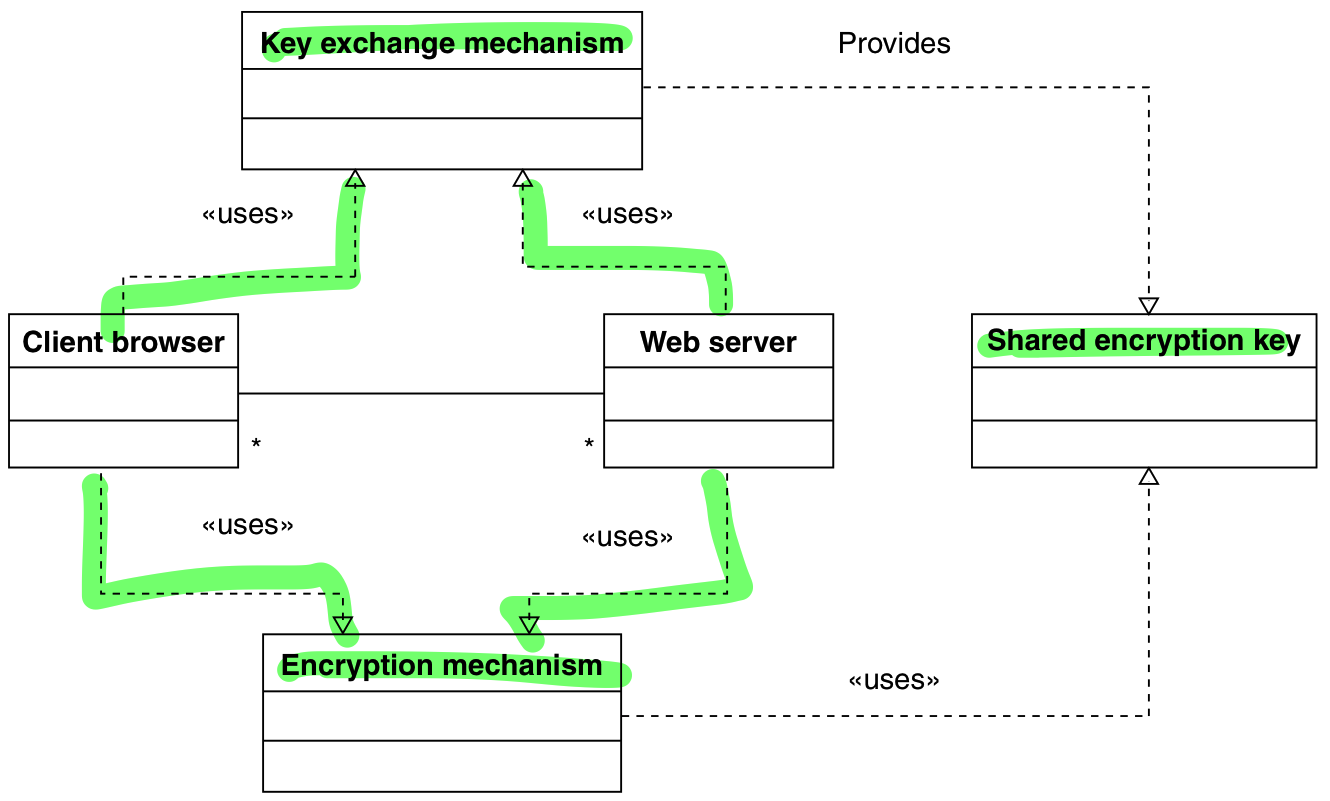
\includegraphics[width=12cm]{content/secure-internet-applications/images/secure-channels-overview.png}
	\caption{Komponenten des Secure Channels Patterns \cite{SecPatterns06}}
\end{figure}

\begin{itemize}
	\item Der \emph{Web server} stellt die eigentlichen Informationen bereit und kann mit dem \emph{Client browser} über einen universalen \emph{Key exchange mechanism} Schlüssel zur gesicherten Kommunikation aushandeln.
	\item Der \emph{Client browser} verfügt ebenfalls über den universellen \emph{Key exchange mechanism} über welchen er mit dem \emph{Web server} das Setup einer gesicherten Verbindung durchführen kann.
	\item Sowohl der Client browser als auch der Web server können auf einen \emph{Encryption mechanism} zugreifen, welcher sie befähigt, mittels dem ausgehandelten \emph{Shared encryption key} einen Secure Channel einzurichten.
\end{itemize}

\subsection*{Beispiel: Secure Socket Layer (SSL)}
Ein heute täglich verwendetes Beispiel bietet SSL. Alle gängigen Browser und Web Server Implementation ermöglichen den verschlüsselten Datenaustausch via dem Secure Socket Layer Protokolls.

Beim Erstellen eines Secure Channels wird dabei zuerst immer ein sogenannter \emph{Session Key} ausugehandelt, welcher zur symetrischen Verschlüsselung von Nachrichten verwendet werden kann:

\begin{figure}[H]
	\centering
	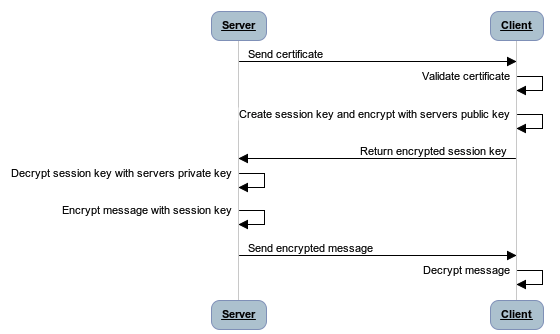
\includegraphics[width=12cm]{content/secure-internet-applications/images/secure-channels-key-exchange.png}
	\caption{Aushandeln eines Session Keys zur sicheren Kommunikation via SSL}
\end{figure}

Dabei fällt auf, dass zur Ermittlung des Session Keys eine asymetrische Verschlüsselung zur Anwendung kommt. Diese benötigt mehr Leistung und kommt aus diesem Grund anschliessend nicht mehr zur Verwendung.

Der Session Key kann mitten in einer aktiven Verbindung ausgewechselt werden. So erschwert man potentiellen Angreifern zusätzlich das dechiffrieren der Nachrichten.


\subsection*{Ergänzungen}
\begin{itemize}
	\item Die Verwendung eines Load Balancers und mehreren Web Servern erschwert die Verwendung eines Secure Channels: Nach dem Aufbauen einer Verbindung zum einen Web Server muss der Load Balancer nicht gezwungener massen bei einem nächsten Request wieder auf den selben Web Server weiterleiten.\\Um dieses Problem zu umgehen kann ein Load Balancer eine Verbindung an einen spezifischen Web Server ``pinnen'', solange die entsprechende SSL aktiv ist.
\end{itemize}

\subsection*{Vorteile}
\begin{itemize}
	\item Die Sicherheit von übertragenen Informationen ist gewährleistet. Sie können auf dem Weg zu ihrem eigentlichen Ziel nicht gelesen werden.
	\item Es ist keine spezifische Software/Hardware notwendig; SSL wird von allen aktuellen Browsern unterstützt.
	\item Durch den Key exchange mechanism ist es möglich, dass sich eigentlich unbekannte Partner einen Secure Channel aufbauen können.
	\item Normale, ungesicherte Kommunikation wird nicht beeinträchtigt.
\end{itemize}

\subsection*{Nachteile}
\begin{itemize}
	\item Die Verwendung eines Secure Channels benötigt an beiden Enden mehr Leistung.
	\item Verschiedene Massnahmen um ein System skalierbar zu machen (Load Balancing) verkomplizieren die Verwendung eines Secure Channels
	\item Erhöhte Wartungskosten, evtl. sogar höhere Anschaffungskosten für Serverhardware um zusätzliche Leistung stellen zu können.
\end{itemize}

\subsection*{Mögliche Prüfungsfragen}
\begin{itemize}
	\item \emph{Warum verwendet nur der Key exchange mechanism eine asynchrone Verschlüsselung?}\\
	Asynchrone Kryptographie Methoden sind aufwändiger zu berechnen. Aus diesem Grund wird lediglich der Session Key für den Secure Channel über diese sicherere Verschlüsselungsmethode übertragen.\\Der Session Key wird während dem Aufrechterhalten des Secure Channels beliebig ausgetauscht um so ebenfalls eine hohe Sicherheit zu gewährleisten.
\end{itemize}